\newpage
\section{Prac 5 - ALU}
\label{sec:Prac5}
\subsection{Overview}
An arithmetic logic unit (ALU) is a digital building block which can perform a variety of arithmetic, logical and bit shift operations. It is the base building block of a central processing unit and operates on integer binary numbers. The unit has both data and control signals. A basic ALU has two parallel input data busses (A) and (B) and one parallel output data bus (Y). It also has a parallel bus (F) which takes in an opcode or binary value which selects a specific arithmetic, logical or shift operation to be performed by the ALU on the two inputs A and B, it may also have a status output bus S which gives more information about the previous operation.\footnote{\textit{Orignal practical by Robyn Verrinder}}
\begin{figure}[H]
\centering
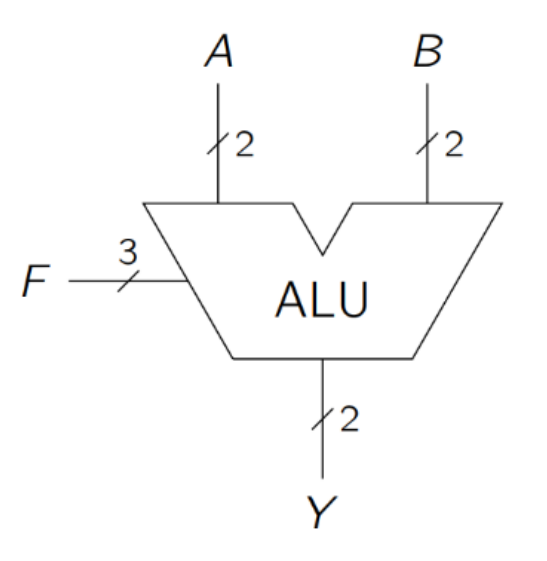
\includegraphics[width=0.35\columnwidth]{Figures/ALU}
\caption{An Example of a simple ALU with a 2-bit wide data bus}
\label{fig:ALU}
\end{figure}

\subsection{Pre-Practical Requirements}
\begin{itemize}
    \item \href{http://www.cburch.com/logisim/}{Logisim}
    \item Understanding of the following components:
    \begin{itemize}
        \item AND Gates 
        \item OR Gates
        \item NOT Gates
        \item XOR Gates 
        \item 1-bit full adders 
        \item 2-input multiplexers (MUX)
    \end{itemize}
    \item There is no pre-prac assosciated with Practical 5
\end{itemize}

\subsection{Tasks}
\begin{itemize}
    \item Design the ALU using the logical building blocks mentioned in the pre-practical requirements. Explain each step in your report. (30) \footnote{This is not a technical report as the one expected in practical 2. However, each building blocks must be represented in a figure, the functionality and the role of each building block in the bigger system must be explained.}
    \begin{itemize}
        \item 3 marks per sub-circuit for each operation. It must include a description of how the circuit works. 6 marks for the interlinking circuits including the multiplexers.
    \end{itemize}
    \item Simulate your design in Logisim. Clearly label all inputs, outputs etc. Export a jpeg of the circuit and include it in your report. (10)
\end{itemize}

\subsection{Deliverables}
\begin{itemize}
    \item At the end of the practical 5, you are to submit one .circ file (simulation file) and one .pdf file including your answers on Vula. The pdf and circ file must have the following format:
    \begin{verbatim}
    prac_<prac_number>_<std_number1>_<std_number2>.<extension>    
    \end{verbatim}
    \item Marks will be deducted for incomplete or untidy reports.
    \item DO NOT COMPRESS THE FILES - Submit two files to Vula
\end{itemize}


\subsection{Further Instructions}
You are required to design and implement a 2-bit wide ALU with a 3 bit opcode, as shown in Table \ref{tbl:Opcodes} below.
\begin{table}[H]
\centering
\caption{Three bit opcode and equivalent operation}
\label{tbl:Opcodes}
\begin{tabular}{|c|c|c|c|c|}
\hline
\multicolumn{3}{|c|}{\textbf{Opcode}} & \multicolumn{2}{c|}{\textbf{Function}} \\ \hline
$F_2$ & $F_1$ & $F_0$ & \multicolumn{2}{c|}{F} \\ \hline
0 & 0 & 0 & A+B & Addition \\ \hline
0 & 0 & 1 & A-B & Subtration \\ \hline
0 & 1 & 0 & A+1 & Increment \\ \hline
0 & 1 & 1 & A-1 & Decrement \\ \hline
1 & 0 & 0 & A $\times$ 2 & Multiply by 2 \\ \hline
1 & 0 & 1 & A $\div$ 2 & Divide by 2 \\ \hline
1 & 1 & 0 & A $\wedge$ B & Bit-wise AND \\ \hline
1 & 1 & 1 & A $\vee$ B & Bit-wise OR \\ \hline
\end{tabular}%
\end{table}